%!TeX root=../tese.tex
%("dica" para o editor de texto: este arquivo é parte de um documento maior)
% para saber mais: https://tex.stackexchange.com/q/78101

\chapter{Introduction}

\section{Reinforcement Learning}
Reinforcement learning is learning what to do in order to maximize reward received. The learner (or "agent") has no knowledge on what actions should be taken, as in many forms of machine learning. Instead, it must discover which ones yield the most reward by trying them and observing what happens. When taking an action, that action may affect not only the immediate reward but also the next reward and all the subsequent others. These two characteristics - trial-and-error search and immediate vs. delayed rewards are the most distinguishing aspects of a reinforcement learning problem. 

The following examples illustrate how reinforcement learning concepts are applied in real life:
\begin{enumerate}
    \item A chess player making a move. The move is informed both by planning - anticipating possible replies and counterreplies - and by intuititve judgements of what positions and moves are desirable.
    \item A gazelle calf struggling to stand on its feet after being born and a few hours later being able to run.
\end{enumerate}

Both examples involve an interaction between a decision-making agent and the environment, in which the agent seeks to achieve a goal, despite uncertainty about its environment. The agent's action may affect the future state of the environment, for example, the next chess move will affect the possible options and opportunities in the future. Taking the correct choice requires taking into account indirect and delayed consequences of actions, and thus requires planning.

Both examples have goals in which the agent can judge the progress towards it based on what it can sense directly. For example, the chess player could judge his progress by comparing his remaining pieces with the opponent's. The player also knows whether he wins.

In order to fully formulate a reinforcement learning problem, we need optimal control of a Markov Decision Process, which will be discussed later, but the basic elements are shown in the next section. 

\section{Elements of a Reinforcement Learning Problem}
Apart from the agent and environment, there are other subelements of a reinforcement learning system: a \textit{policy}, a \textit{reward signal}, a \textit{value function} and, optionally, a \textit{model of the environment}.

A \textit{policy} is a mapping from perceived states to actions to be taken when in those states, that is, a policy is what defines the agent's behavior. Policies can be deterministic, being a simple function or a lookup table, or stochastic, with probabilities associated with each action.

A \textit{reward signal} is what defines the goal in a reinforcement learning problem. At each time step, the environment sends a reward signal, which is just a number. The agent's goal is to maximize reward received over the long run. In biological systems, rewards are analogous to feeling pleasure or pain. The reward received depends on the agent's current action and on the state of the environment. The agent cannot alter this process in any way, but it can influence it through its actions. The reward signal is the primary basis for altering a policy. If an action selected by the policy yields a low reward, then the policy may be changed to select another action in that situation in the future.

A \textit{value function} tells us how much reward the agent should expect to receive over the future by starting in a specific state. While reward signals indicates whether a state is immediately desirable or not, the value function estimates the long-term desirability of that state by taking into account the states that are likely to follow the current one. For example, a low reward state might be followed by a high reward state or vice versa. It's values we are most concerned with when making and evaluating decisions - we seek for actions that yield maximum value, not reward. Note that this is equivalent to maximizing reward over the long run. The major problem with value is that it can be hard to estimate - rewards are given directly by the environment, but values must be re-estimated at each iteration from sequences of observations an agent makes over its lifetime. The most important component of almost all reinforcement learning algorithms is value function estimation.

A \textit{model of the environment} is something that mimics the behavior of the environment itself. More generally, that allows for inferences about how the environment will respond to certain actions. For example, for a given pair of state and action, the model might predict how the environment will respond to that action in that particular state. Models are particularly useful for \textit{planning}, which is deciding on a course of action by considering possible future situations. Methods that use models and planning are called \textit{model-based} methods, as opposed to \textit{model-free} methods that rely on trial-and-error to learn about the environment.

\section{Agent-Environment Interface}
The learner and decision-maker agent and the thing it interacts with, comprising of everything outside the \textit{agent}, is defined as the \textit{environment}. The agent and the environment interact continually, with the agent choosing actions and the environment responding to those actions, presenting new situations to the agent and rewarding it.

\begin{figure}[H]
    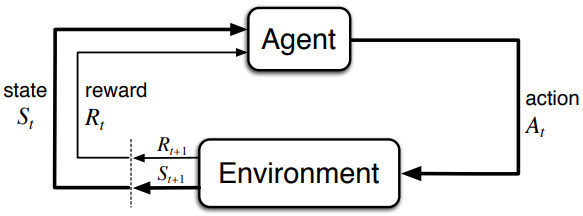
\includegraphics[width=\textwidth]{agent-environment}
    \caption{Representation of the agent-environment interface from \cite{suttonbarto}.}
\end{figure}

In other words, at each time step $t = 0, 1, 2, \dots$, the agent receives some representation of the environment's state $S_t \in \mathcal{S}$, where $\mathcal{S}$ is the set of all possible states, and selects an action $A_t \in \mathcal{A}(S_t)$, where $\mathcal{A}$ is the set of all possible actions and $\mathcal{A}(S_t)$ the set of all possible actions in state $S_t$. At the next time step $t+1$, the agent receives a reward $R_{t+1} \in \mathbb{R}$ and a new state $S_{t+1}$. 

The action the agent takes is sampled from the agent's policy, denoted $\pi$, with $\pi(a \mid s)$ being the probability of taking action $a$ when in state $s$. $\pi$ is just an ordinary function defining a probability distribution over $a \in \mathcal{A}(s)$. Reinforcement learning methods specify how the policy is changed as the agent gathers more experience. 

\section{Goals and Rewards}
The goal of an agent is formalized in terms of a reward signal $R_t \in \mathbb{R}$ that is passed to the agent by the environment. Consider the sequence of rewards received after time step $t$: $R_{t+1}, R_{t+2}, \dots$. We define a \textit{return} $G_t$, which is a function of that sequence. The simplest case is the sum of all of them:
\[
    G_t = R_{t+1} + R_{t+2} + \dots + R_T
\]
The agent's goal is to maximize the total amount of rewards it receives. In other words, the goal is to maximize the \textit{expected return} $\mathbb{E}[G_t]$. In the above definition, we have the notion of a final time step, which comes very naturally when the agent-environment interaction can be broken down into subsequences, which we call \textit{episodes} or \textit{trials}. For example, plays of a game, trips through a maze or any sort of repeated interactions can be considered episodes. Each episode ends in a special state called \textit{terminal state}, followed by a reset to a standard state or to a sample of a distribution of starting states.

However, not all agent-environment interactions can be breaked naturally into episodes, instead, it could go on without limit. That is, with slight abuse of notation, $T = \infty$ and the return $G$ could easily be infinite as well. Thus, the concept of \textit{discounting} arises, where we introduce a \textit{discounting factor} $\gamma$, $0 \leq \gamma \leq 1$, to weigh immediate and future rewards:

\[
    G_t = R_{t+1} + \gamma R_{t+2} + \gamma^2 R_{t+3} + \dots = \sum_{k=0}^{\infty}\gamma^k R_{t+k+1}
\]

Then, the sum is finite as long as $\gamma < 1$ and the reward sequence is bounded. Also note that if $\gamma = 0$, the agent is only concerned with immediate rewards and the action $A_t$ will be chosen in such a way to maximize only $R_{t+1}$. If $\gamma$ is close to $1$, then the future rewards will be taken into account more strongly.

According to \cite{suttonbarto}, although formulating goals in terms of reward signals appears to be limiting, in practice, it has proved to be flexible and widely applicable. For example, to make a robot learn how to escape from a maze, the reward is often -1 for every time
step that passes prior to escape; this encourages the agent to escape as quickly as possible.

While designing how rewards should be given to the agent, it's crucial that it's done in such a way maximizing also makes the agent achieve the goal. That is, the reward signal must not be used to impart any prior knowledge to the agent about how to achieve the goal. For example, in a chess game, rewards should be given when the agent wins the game, and not when accomplishing subgoals, such as taking enemy pieces. If the agent gets rewarded for achieving subgoals, it might find a way to maximize the rewards by only taking enemy pieces and without actually winning. All in all, the reward signal is our way of communicating to the agent what needs to be done, not how to do it. 